\section{Einleitung}
	\subsection{Forschungsfrage und Zielsetzung}
	Seit dem 30. November 2023 ist der Chatbot ChatGPT veröffentlicht und frei nutzbar. 
	Nur nach weniger als zwei Monaten hatte ChatGPT bereits 100 Millionen Nutzer \cite[S. 15]{spitzer23}.
	Wegen des großen Erfolges begannen schon nach kurzer Zeit weitere Unternehmen wie Google ihre eigenen 
	Chatbots zu entwickeln. Mitlerweile gibt es immer umfangreichere sowie leistungsfähigere KI und
	deren Entwicklung schreitet unglaublich schnell voran.
	
	Diese Technologie hat einen immer größer werdenden Einfluss auf unsere moderne Gesellschaft. 
	Chatbots sind für viele Menschen bereits Teil ihres Alltags und helfen in der Schule oder
	im Studium, aber auch im Beruf, beispielsweise dann, wenn es darum geht längere Texte zu verfassen \cite[S. 175, S. 185]{shaji23}.
	Auf der andere Seite gibt es sogar Chatbots die keinen praktischen Nutzen haben und dazu gedacht
	sind, dass man sich mit ihnen die Zeit vertreibt, indem man z. B. emotionale gespräche mit ihnen 
	führt. Diese Art der Chatbots sollen als eine art KI Fruend dienen, sie sind vor allem in form
	von Anwendungen aus dem Play Store \& App Store bekannt.
	
	Es ist wichtig so eine Technologie richtig einordnen zu können. Jedoch wissen die wenigsten
	wie Chatbots funktionieren, was dazu führt, dass deren fähigkeiten oft flasch eingeschätzt werden. 
	Darum soll in dieser Arbeit der Frage nach gegangen werden, welches Bild die Offentlichekeit von 
	Chatbots hat, bzw. was an diesem Bild problematisch sein kann. 

	Diese Arbeit verfolgt das Ziel aufzuzeigen, welcher Eindruck von Chatbots in den Medien   
	vermittelt wird. Daraus sollen Schlüsse gezogen werden, wie Öffentlichkeit über KI denkt.  
	Außerdem soll die Arbeit verständlich erklären, warum der Eindruck von Chatbots bzw. KI oft 
	fehlerhaft ist. Dazu wird näher auf die Funktionsweise dieser Programme eingegangen. Nach 
	dem Lesen der Arbeit soll man ein grundlegendes Verständnis von Chatbots haben und mit 
	Informationen diesbezüglich aufgeschlossener umgehen können. 

	\clearpage
	\subsection{Methodik und Aufbau} 
	Im ersten Teil der Arbeit werden verschiedene Beispiele behandelt, die zeigen, dass leicht ein falscher 
	Eindruck von KI, insbesondere Chatbots, vermittelt wird. Zunächst wird auf die soziale Bedeutung bestimmter
	KI-Chatbots eingegangen, und die damit verbundenen Konsequenzen und Folgen werden genauer erläutert. Anschließend
	wird anhand populärwissenschaftlicher Artikel aufgezeigt, dass die Funktionsweise von KI häufig missverständlich 
	oder ungenau dargestellt wird, was in solchen Quellen leicht zu Missverständnissen führen kann.
	Daraufhin erfolgt eine grundlegende Betrachtung des Themas Chatbots und IQ-Tests. Zunächst wird erläutert, welche
	Bedeutung IQ-Tests im Zusammenhang mit Chatbots haben. Des Weiteren wird gezeigt, was man bei der Auswertung von 
	Ergebnissen, die Chatbots erziehlen, beachten muss.

	Der zweite Teil der Arbeit beschäftigt sich mit der Funktionsweise von Chatbots. Zunächst werden einige wichtige Begriffe
	geklärt, gefolgt von einer Einführung in das LLM und den GPT. Die grundlegende Funktionsweise von KI-Chatbots wird dabei 
	leicht verständlich vermittelt. Mit diesem neuen Wissen wird anschließend das Thema AGI\footnote{Artificial General Intelligence} behandelt. 
	Anhand ausgewählter Beispiele wird verdeutlicht, warum zum gegenwärtigen Zeitpunkt noch keine AGI entwickelt wurde. Das Thema AGI ist hier 
	besonders relevant, da im ersten Teil der Arbeit bereits gezeigt wurde, dass moderne KI häufig falsch dargestellt wird und die Unterscheidung 
	zwischen AGI und ANI\footnote{Artificial Narrow Intelligence} oft schwerfällt.

	Im abschließenden Teil der Arbeit sollen Missverständnisse und Problematiken aus dem ersten Teil geklärt werden. Zunächst wird 
	darauf hingewiesen, dass KI derzeit weder intelligent ist noch menschliche Gefühle oder Emotionen besitzt. Anschließend werden 
	Missverständnisse aus den zuvor behandelten Artikeln aufgeklärt. Abschließend wird die Problematik von IQ-Tests, die von Chatbots 
	bearbeitet wurden, diskutiert. 	
	
	
\clearpage
\section{Die öffentliche Wahrnehmung von Chatbots}\label{s1}
	\subsection{Chatbots mit Gefühlen?}\label{s1ss1}
	Eine kurze Erklärung vorab: Die meisten kennen vermutlich bekannete Chatbots wie ChatGPT, die dazu
	entwickelt wurden uns bei diversen Aufgaben zu unterstützen. Im Gegensatz dazu steht Character.AI, 
	eines der Unternehmen, die \glqq{}persönliche\grqq{} AEI\footnote{Artificial Emotional Intelligence} 
	anbieteten \cite{cAI24}. Das bedeutet, dass die KI dazu entworfen wurde, soziale Gespräche zu führen.
	Man kann zwischen verschiedenen Chatbots, die meist fiktive Charaktäre räpresentierten, wählen. Sie
	sind darauf ausgelegt möglichst emotional und menschlich zu reagieren und oft stehen dabei sehr 
	persönliche Themen im Vordergrund, z. B. Einsamkeit, Freundschaft, Empathie oder sogar Liebesbeziehungen. 
	
	Das dabei eine emotionale Verbindung zu Chatbots entstehen kann ist durchaus möglich und dafür reicht ein 
	Chatbot aus, der nur begrenzte soziale Fähigkeiten hat \cite{chen24}. KI ist für viele Menschen also 
	nicht nur eine parktische Anwendung, die im Alltag hilfreich ist, sondern hat für einige Personen auch
	emotionalen Mehrwert. Ob und wieso das Kritisch gesehen werden muss wird \ref{s3ss1} diskutiert.  

	Character.AI ist nur eines von mehreren Unternehmen, die persönliche AEI anbieten, und das mit Erfolg. 
	Seit September 2022 ist Character.AI frei verfügbar und hat zum jetzigen Zeitpunkt August 2024 bereits
	über 10 Millionen Downloads bei Google Play. Auf Grund der schnellen Weiterentwicklung von KI und des 
	global stärker werdenden Gefühls von Einsamkeit ist demnach zu erwarten, dass die soziale Bedeutung 
	von Chatbots zunehmen wird \cite{chen24}. 
	
	
	\clearpage		
	\subsection{Mediale Berichterstattung}\label{s1ss2}
	Die Medien spielen bei der Berichterstattung über KI eine entscheidende Rolle. Sie tragen nicht nur dazu
	bei, die Öffentlichkeit über aktuelle Entwicklungen und Innovationen zu informieren, sondern sind auch 
	verantwortlich dafür, komplexe technische Zusammenhänge verständlich zu vermitteln. Doch genau hier kann
	es auch zu Problemen kommen, wodurch eine falsche Auffassung von aktuellen Chatbots entsteht.

	Ein beispiel hierfür ist das Demonstrationsvideo von Google zu ihrem Chatbot Gemini \cite{gminiDemo2023}. 
	Das Video zeigt eine Person, die mit dem Chatbot Gemini live interagiert und ihm Fragen stellt. Dabei
	zeichnet die Person beispielsweise ein Bild von einer Ente und stellt dem Chatbot immer wieder Fragen dazu.
	Später im Video deutet die Person durch handbewegungen an, dass sie mit dem Chatbot das Spiel \glqq{}Schere
	Stein Papier\grqq{} spielen will. Der Chatbot antwortet, dass er die Herausforderung annimmt. Das Video
	betont damit vor allem die Interaktivität zwischen Gemini und der anwesenden Person. Außerdem zeigt das
	video einen autonomen Chatbot, der aus einem bestimmten Context Schlüsse zieht, welche Antwort gefragt ist. 

	In vielen Artikeln zu Chatbots wird deren Funktionsweise und Training erklärt. Maria Gramsch erklärt in 
	ihrem Artikel wie ChatGPT funktioniert. Sie fasst sich hierbei kurz und erklärt unteranderem
	auch das Training von Chatbots. In dem Artikel ist zwei mal zu lesen, dass das Trainig von ChatGPT stets
	unvollendet ist und dass der Chatbot aus Konversationen mit den Nutzern immer weiter dazu lernt \cite{gramsch23}. 
	Dadurch wird der Eindruck vermittelt, dass ChatGPT wie ein Mensch aus seinen Erfahrungen lernt.

	Was genau an den gennanten Beispielen zur Berichterstattung falsch ist wird in \ref{s3ss2} verdeutlicht. 
	Es steht aktuell eine Vielzahlt an Möglichkeiten zur Verfügung, um sich über KI und Chatbots zu informieren. 
	Dadurch kann es schwirig werden eine passende Informationsquelle zu wählen, die gut verständlich ist.   	 	 
	
	\clearpage
	\subsection{Chatbots und IQ-Tests}\label{s1ss3}
	Mit der steigenden Zahl an KI Modellen, wird KI-Benchmarking\footnote{Verglich von KI-Systemen} immer wichtiger. 
	Außerdem stellt sich die Frag, wie Intellegent ein Chatbot verglichen mit einem Menschen ist. IQ-Tests 
	bieten eine Möglichkeit das zu tun, sie sind dazu entworfen Intellegenz so gut wie möglich zu messen und das 
	funktioniert auch bei KI. Jedoch ist es wichtig die Ergebnisse, welche KI in IQ-Tests erzielt, kritisch zu
	sehen und richtig zu deuten.

	Eka Roivainen schreibt in ihrem Artikel, wie er mit dem damals neu veröffentlichten ChatGPT-4 einen IQ-Test
	durchgeführt hat \cite{roivainen23}. Sie schildert zu beginn des Artikels, dass sie sich dafür interessiere, wie
	schlau ChatGPT im Vergleich zu menschlichen Standarts ist. Im verbalen Teil des verwendeten WAIS-III Tests
	erklärt sie, der Chatbot hat einen Wert von 155 erzielt und ist damit besser als 99,9\% der menschliche Teilnehmer.
	Der Artikel wurde mehreren anderen Artikeln zitiert, wie beispielweise von Sandra Blütermann in ihrem Artikel
	\cite{blutermann23}. In einem Interview von Sky News Australia erklärt Mo Gawdat ein ehmaliger Chief Business
	Officer von Google ebenfalls, dass ChatGPT einen IQ von 155 habe und damit fast so intellegent wie Alber Einstein
	sei \cite{gawdat23}.

	Betrachtet man das Ergebnis, was Roivainen mit ChatGPT-4 in ihrem IQ-Test erziehlt hat könnte man meinen,
	dass KI dem Menschen bereits überlegen ist. Mo Gawdat sagt das sogar schon fast wörtlich in seinem Interview:
	\glqq{}Der IQ von ChatGPT-4 wird auf 155 geschätzt, das ist viel schlauer als der durchschnittliche Mensch\grqq{} 
	\cite{gawdat23}. In \ref{s3ss3} werden die Ergebnisse, von ChatGPT-4 im WAIS-III Test genaur betrachtet.
	Darüber hinaus wird die Aussage von Mo Gawdat über die Intellegenz von ChatGPT-4, diskutiert und widerlegt. 	

\clearpage	
\section{Die Funktionsweise von KI-Dialogsystemen}
	\subsection{Begriffe und Grundlagen}\label{s2ss1}
	Um das nächste Kapitel verstehen zu können, müssen zunächst einige wichtige Begriffe und Sachverhalte erklärt 
	werden. Natürlich kann im Rahmen dieser Arbeit nicht eine komplette Erklärung rund um LLM und GPT bis ins Detail
	gewährleistet werden, darum beziehe ich mir hier auf das Nötigste, um die folgenden Teile der Arbeit gut verstehen
	zu können: 
	
	\begin{itemize}
		\item \textbf{Neuronale Netze}: Man kann ein neuronales Netz als eine Mathematische Funktion sehen,
		die eine Anzahl $n$ an Werten annimt und eine Anzahlt $m$ an Werten ausgibt. Diese Werte kann man auch als Eingabe-
		und Ausgabevektor sehen: 		
		
		\begin{equation*}	
			f(\vec{v}) = \vec{w}\textnormal{,\qquad wobei } \vec{v} \in \mathbb{R}^n \textnormal{ und } \vec{w} \in \mathbb{R}^m
		\end{equation*}  
		\vspace{0.0cm}
		
		Die Funktion $f$ hat zahlreiche Parameter (175 Milliarden bei GPT-3 \cite[S. 8]{openAI2020}), die man genau so 
		anpassen will, dass aus unterschiedlichen Eingabevektoren die gewünschten Ausgabevektoren werden und genau hier kommt 
		das Training ins Spiel. Durch Training ist es möglich die Zahlreichen Parameter des Netzwerks so einzustellen, dass 
		sich die Werte der Ausgabevektoren möglichst gut an die gewünschten Werte annähern \cite[S. 127f]{nielsen2015}. Bei
		der Verwendung eines neuronalen Netzwerks findet kein Training statt.   

		\item \textbf{Schicht eines Neuronalen Netzwerks}: In einem neuronalen Netzwerk gibt es mehrere Schichten, die einzelne
		Bearbeitungsschritte darstellen. Die Eingabevektoren durchlaufen jede Schicht und werden dabei in die Ausgabevektoren
		umgerechnet \cite[S. 4]{nielsen2015}. 
		
		\item \textbf{NLP}: Natural Language Processing ist ein Feld der KI, dass darauf spezialisiert ist natürliche 
		Sprache zu analysieren, transformieren oder zu generieren.  
		
		\item \textbf{LLM}: Ein Large Language Model ist, wie der Name schon sagt ein großes KI Model unserer Sprache.
		LLMs sind auf NLP spezialisiert und funktionieren unter der Verwendung von Neuronalen Netzen.

		\item \textbf{Transformer}: Die Transformerachitektur ist ein neuronales Netzwerk-Modell, das erstmals im 
		bekannten Forschungsartikel \glqq{}Attention is all You Need\grqq{} von Forschern bei Google vorgestellt wurde 
		\cite{vaswani2017}. Transformer in Verbindung mit Chatbots werden in \ref{s2ss1} genauer erklärt.
		
		\item \textbf{GPT}: Ein Generative Pre-Trained Transformer ist ein LLM das sich die Transformerachitektur 
		zu Nutze macht um ein deutlich besseres Ergebnis bei der Sprachverarbeitung zu erzielen. Diese GPTs sind
		der Grund für den Fortschritt im Bereich NLP und sie werden derzeit in fast allen bekannten Chatbot Modellen, 
		wie ChatGPT und Gemini verwendet \cite[S. 2]{gemini2024}, \cite[S. 1]{openAI2024}.  
		
		\item \textbf{Token}: Wenn ein Chatbot eine Nachricht verarbeitet, dann wird diese zunächst in mehrere kleinere 
		Tokens zerlegt. Tokens helfen bei der Sprachverarbeitung, indem sie Zeichenfolgen in Wörtern darstellen \cite{mielke2021}.  
		Zur vereinfachung kann man sich auch vorstellen, dass ein Token ein Wort räpresentiert.   
	\end{itemize}	
	\clearpage
	
	
	\subsection{Transformer und Chatbots}\label{s2ss2}
	Im Folgenden wrid der schematische Aufbau eines Transformers erklärt. Wie schon in \ref{s2ss1} erwähnt wurde 
	ist ein Transformer ein neuronales Netzwerk-Modell. Das heißt der Transformer nimmt einen Vektor an rationalen 
	Zahlen als Eingabe und gibt ebenso einen Vektor aus.      	
	
	\tikzstyle{concept} = [rectangle, rounded corners, minimum width=2cm, minimum height=0.8cm, text centered, draw=black, fill=orange!40, line width = 0.5mm]
	\tikzstyle{arrow} = [thick,->,>=stealth, line width = 0.5mm]
	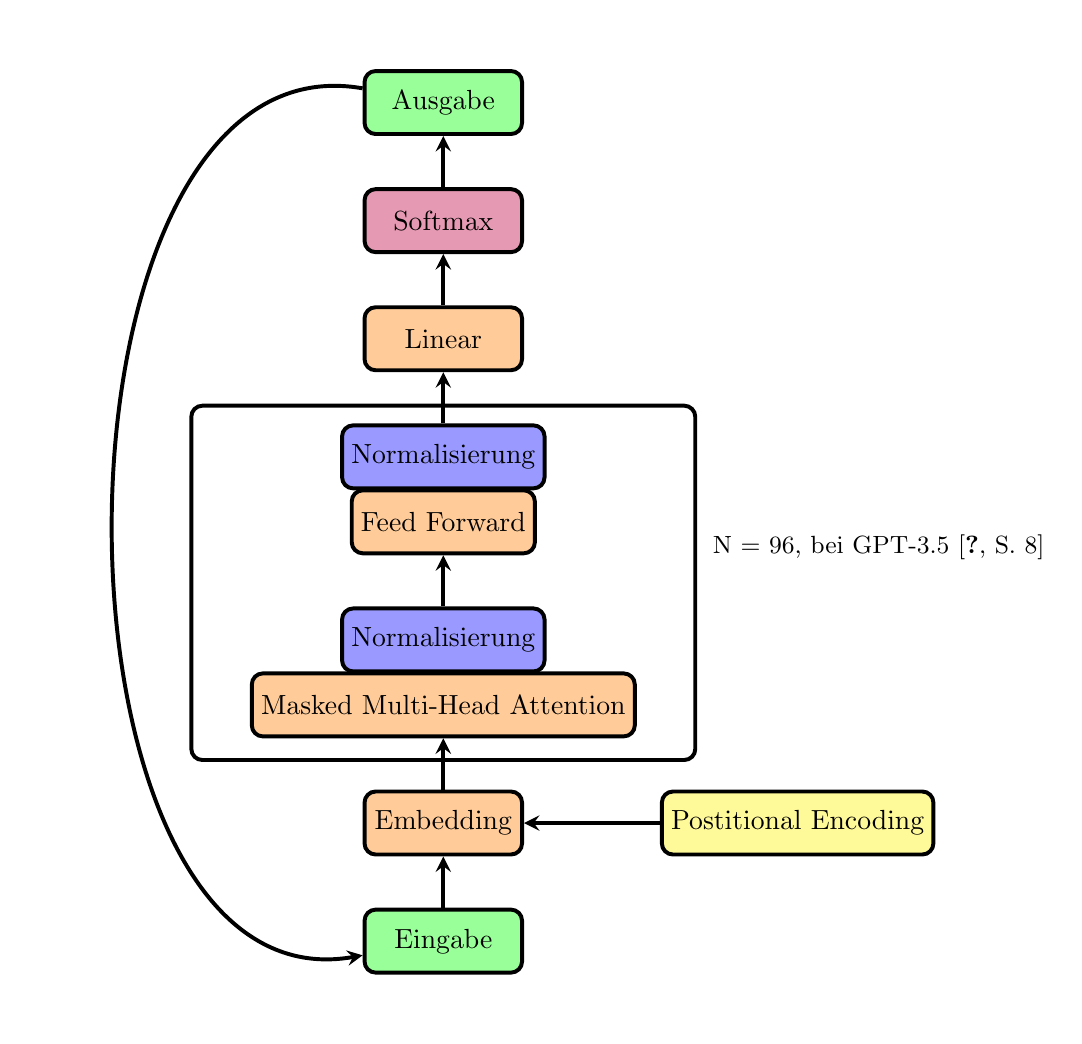
\begin{tikzpicture}[node distance=1.5cm]
		% Nodes
		\node (input) [concept, fill=green!40] {Eingabe};
		\node (embedding) [concept, above of=input] {Embedding};
		\node (encoding) [concept, right of=embedding, fill=yellow!40] (encoding) at (3, 1.5) {Postitional Encoding};
		\node (attention) [concept, above of=embedding] {Masked Multi-Head Attention};
		\node (normal) [concept, above of=attention, fill=blue!40] at (0, 2.325) {Normalisierung};
		\node (forward) [concept, above of=normal] {Feed Forward};
		\node (normal1) [concept, above of=forward, fill=blue!40] at (0, 4.65) {Normalisierung};
		\node (linear) [concept, above of=normal1] {Linear}; 
		\node (softmax) [concept, above of=linear, fill=purple!40] {Softmax};
		\node (output) [concept, above of=softmax, fill=green!40] {Ausgabe};
		% Arrows
		\draw [arrow] (input) -- (embedding);	
		\draw [arrow] (encoding) -- (embedding);
		\draw [arrow] (embedding) -- (attention);
		\draw [arrow] (normal) -- (forward);
		\draw [arrow] (normal1) -- (linear);
		\draw [arrow] (linear) -- (softmax);
		\draw [arrow] (softmax) -- (output);
		\draw [arrow, bend right=100] (output) to (input);
		\draw[rounded corners, line width=0.5mm] (-3.2, 2.3) rectangle (3.2, 6.8);  
		\node[right] at (3.3, 5) {\small{N = 96, bei GPT-3.5 \cite[S. 8]{openAI2020}}};
		%\draw [highlight] (input) -- ++(-1,1) -- ++(4,0) -- ++(0,-2) -- cycle;
	\end{tikzpicture}
	
	
	Die erste Aufgabe eines Chatbots ist es also Text zunächst in einzelne Tokens aufzuteilen und dann disen Tokens 
	einen individuellen Vektor zu zu ordnen. Das wird auch als Embedding bezeichnet. Durch das unwandeln von Tokens in 
	einen Vektor kann das Netzwerk Text mathematisch verarbeiten. Weil die einzelnen Tokens nicht der Reihe nach sondern 
	unabhängig von einander und parallel zu einander verarbeitet werden, muss deren Position im Satz mit in den Eingabevektor 
	encodiert werden \cite[S. 2f]{vaswani2017}. Das liegt daran das bei vielen Wörtern die Position im Satz eine 
	Entscheidende Rolle dafür spielt, was der Satz aussagt:

	\vspace{3mm}
	\emph{Der Mann jagt den Hund.} 	
	\space $\neq$ \space
	\emph{Der Hund jagt den Mann.}
	
	\clearpage
	\noindent
	Die grundlegende Funktionsweise besteht darin, dass der Transformer diese Tokens in Zahlen umwandelt, verarbeitet und dann 
	als Ausgabe errechnet, welches Token mit welcher Wahrscheinlichkeit als nächstes folgt. Natürlich wäre ein Chatbot der nur
	ein Token als Antwort geben könnte ziemlich nutzlos. Das Problem ist aber einfach zu lösen, indem man dem Transformer
	die Tokens der vorherigen Eingabe und dazu die neu generierten Tokens gibt. Das wird auch als Selbstregression bezeichnet und 
	bedeutet, dass der Transformer seine Ausgabe wieder als Eingabe verwendet \cite[S. 2]{vaswani2017}.  

	Nach dem Embedding folgt die eine Masked Multi-Head Attention Schicht\footnote{Teil eines neuronalen Netzwerks}.
	Im fall eines generativen Transformers wird sich hier der  Self-Attention Mechanismus zunutze gemacht \cite[S. 2f]{turner2024}. 
	Dabei wird zunächst errechnet wie stark der Zusammenhang zwischen zwei Tokens ist \cite[S. 4]{vaswani2017}. Hat man zu 
	Beispiel die Frage, \emph{Wie nennt man ein großes Haus?} als Eingabe, könnten die errechneten Zusammenhänge für das 
	Wort Haus so aussehen: 
	
	\vspace{5mm}
	\begin{tabular}{ |c|c| }
  		\hline
	  	\multicolumn{2}{|c|}{Zusammenhang mit Haus: } \\
	  	\hline
	  	\emph{Wie} & 0,046 \\
	  	\hline
	  	\emph{nennt} & 0,08 \\
		\hline
	  	\emph{man} & 0,023 \\
	  	\hline
		\emph{ein} & 0,12 \\
	  	\hline
		\emph{großes} & 0,7 \\
	  	\hline
		\emph{haus} & 0,031 \\
		\hline
		\emph{?} & 0,001 \\
		\hline
	\end{tabular}
	\vspace{5mm}
	
	\noindent Weil sich das Adjektiv \emph{großes} auf das Nomen \emph{Haus} bezieht erkennt ein trainierter Transformer hier
	einen starken Zusammanhang. Durch diese errechneten Zusammenhänge zwischen den Tokens kann das Netzwerk abwägen, welches
	Token auf welches andere Token wie viel einfluss nehmen soll.	
		
	Nach der Multi-Head Attention folgt eine Normalisierung, welche dabei hilft die Vektoren zu verarbeiten. 
	Normalisirungen sind zwar Teil der Transformerachitektur aber nicht entscheidend für ein schematisches Verständnis
	und werden hier nicht genauer beschrieben\cite[S.3]{vaswani2017}. 
	\clearpage
	\noindent
	Der zweite bedeutende Teil eines Transformers folgt direkt auf den attention Block und nennt sich Feed Forward Block.
	Im Feed Forward Block befinden sich c.a. zwei drittel der Parameter \cite{geva2024}. Parameter bestimmer bekanntlicher weise
	die Ausgabewerte einer Funktion oder eines neuronalen Netzwerks. Im Fall eines Chatbots bestimmen diese Paramter, wie auf 
	einen Satz den der Transformer als eingabe bekommt geantwortet wird. Bei diesen Antworten reicht es meistens aber nicht aus, 
	einfach nur Zusammenhänge zwischen Wörtern zu erkennen, wie oben erklärt, sondern man bennötigt Hintergrundwissen zum Thema 
	für eine konstruktive Antwort.

	Im obigen Satz muss man zum Beispiel nicht nur verstehen, das es um ein \emph{großes Haus} geht sondern auch wissen welche alternativen
	Wörter es dafür gibt, um die Frage zu beantworten. Dafür braucht man den Feed Forward Block, er kann als Gedächnis des Transformers gesehen
	werden. Da sich hier ein großteil der Parameter befindet ist hier auch ein großteil des Wissens bzw. der Datan, die ein neuronales
	Netzwerk gelernt hat gespeichert \cite{geva2024}.
	\vspace{5mm}
	Im Attention Block werden also zusammenhänge zwischen den Tokens erkannt und dann Informationen zwischen den Tokens übertragen
	und im Feed Forward Block wird dann noch auf die eingehenden Tokens mit bestimmten issen, welches das Netzwerk besitzt reagiert.
	
	Wichtig ist, dass dieser Ablauf von Attention und Feed Forward in einem Transformer mehrmals wiederholt wird, damit auch längere komplexe Texte mit
	komplizierten Zusammenhängen sinnvol verarbeitet werden können.
	
	Am Ende des Transformer befinden sich noch eine Lineare und eine Softmax Schicht. Sie sind dazu dar die Ausgabe des Transformers
	in einen Vektor zu überführen, der allen definierten Tokens eine Wahrscheinlichkeit zuweist \cite[S. 70]{nielsen2015}. Darunter wählt man dann meist das Token 
	mit der höchsten Wahscheinlichkeit aus und fügt es dem Text hinzu. Diesen Prozess wiederholt man dann so lange, bis der Transformer
	ein EOS-Token\footnote{End-of-Sequence-Token} generiert und damit den Abschluss seiner Antwort signalisiert \cite[S. 2]{vaswani2017}.
	
	
	%chat gpt 3.5 tech report oder specs finden
	%aggarwal2018?
	\subsection{Warum ist das noch nicht AGI?}\label{s2ss3}
	Bei AGI handelt es sich um eine form von KI, die noch nicht existiert. Bis jetzt verwenden wir ausschließlich 
	ANI, dass ist KI die für spezifische Aufgabe, wie z. B. Bilderkennung entwickelt wurde. In \ref{s1} wurde 
	herausgearbeitet, dass jedoch oft der Eindruck vermittelt wird, es handele sich bei modernen Chatbots um 
	eine form von AGI. Im Folgenden wird also herausgearbeitet wieso es sich bei den aktuellen Chatbots um ANI 
	handelt. Allgemein muss eine KI bestimte Eigenschaften erfüllen, um als AGI bezeichnet werden zu können 
	\cite[S. 8]{goertzel23}:
	\begin{itemize}
	\item Eine AGI muss fähig sein ein breites Spektrum an Aufgabe unter verschiedenen Vorraussetzugen zu erledigen. 
	\item Eine AGI sollte auch mit Situationen oder Problemen umgehen können für die sie nicht spiziell entwickelt wurde. 
	\item AGI Systeme besitzen die Fähigkeit gelerntes Wissen von einem Problem auf ein anderes zu transferieren. 
	\end{itemize}	
	Zunächst einmal ist ein moderner Chatbot fähig verschiedenste Aufgabe zu erledigen. Man könnte auch argumentieren,
	dass durch die Bildverarbeitung und Tonverarbeitung, die diese Chatbots oft bereitstellen, verschiedene Vorraussetzungen 
	gelten, unter denen ein Chatbot seine Aufgaben erledigt. Die übrigen zwei Aspekte werden jedoch nicht erfüllt. 
	
	LLMs sind nicht oder nur begrenzt in der Lage mit Problemen um zu gehen, die über das verarbeiten von Text hinaus gehen. 
	Beispielsweise zeigt Ben Goertzel in seiner Arbeit, dass LLMs ein sehr begrenztes räumliches Vorstellungsvermögen haben 
	\cite[S. 32-35]{goertzel23}. Wenn Chatbots fragen, die ein solches Vorstellungsvermögen verlangen, richtig beantworten 
	wird meistens nur auf gelerntes Wissen zurück gegriffen, d.h. das LLM weis die Antwort auswendig.
	
	Letzendlich fehlt mordernen Chatbots vor allem die Fähigkeit erlerntes Wissen auf andere Probleme zu übertragen. Goertzel schreib in
	seiner Arbeit hierzu, dass ein Sprachmodell sein Wissen lediglich als Fallbeispiel abspeichert. Das führt dazu das diese Wissen
	zwar je nach bedarf abgerufen werden kann, aber nicht sinvoll auf andere Situationen transferiert wird. LLMs fehlt eine 
	abstrakte Repräsentation des gelernten Wissens \cite[S. 81f]{goertzel23}. 
	
	\noindent{}Insgesamt ist man sich einig, dass es sich bei LLMs wie ChatGPT oder Gemini nicht um AGI handelt. Auch wenn nach außen
	hin oft der Eindruck vermittelt wird, man spräche mit einer allgemienen intellegenten System, ist das nicht der Fall. 
	
	
\clearpage
\section{Was folgt daraus?}\label{s3}
	\subsection{Nur Algorithmen ohne Gefühle}\label{s3ss1}
	In \ref{s1ss1} wurde bereits gezeigt, dass KI Chatbots in der Gesellschaft teils mehr als nur nützliche Assistenten sind.
	Jedoch muss die soziale Nutzung von Chatbots kritisch gesehen werden. Dafür gibt es folgende Gründe:

	Zunächst ist es wichtig zu verstehen, dass aktuelle Chatbots keine gefühle empfinden, auch wenn es nach außen hin so wirkt.
	Wie bereits in \ref{s2ss2} gezeigt wurde handelt es sich bei modernen Chatbots um LLMs, also Programme, die durch berechnung
	Texte generieren. Das LLM wird zunächst anhand von beispieltext trainiert. Will man also, dass ein Chatbot fähig ist ein
	soziales gespräch zu führne würde man ihn beispielsweise mit passenden Chatverläufen trainieren. Dadurch lernt der Chatbot
	zwar während sozialen Konversationen eine passende Antwort zu geben, jedoch versteht er dessen bedeutung nicht \cite[S. 35-38]{goertzel23}.
	Das heißt also, dass Chatbots lediglich anhand von trainigsdaten lernen so zu tun als hätten sie Gefühle. 

	Abgesehen von der Tatsache, dass Chatbots nicht in der Lage sind Gefühle zu empfinden, kann die vermehrte Nutzung von KI anstelle
	des Menschen zu einer Entmenschlichung führen. Indem man einem Chatbot menschliche Eigenschaften zuschreibt und Programme auf
	das gleiche Level wie reale Menschen stellt, verliert die soziale Interaktion mit echten Menschen an Bedeutung. Außerdem wird die
	soziale Komponente des Menschen dadurch ersetzbar gemacht, wordurch sie an Wert verliert \cite{chen24}. 	 

	Natürlich gibt es auch positive Aspekte, die eine Nutzung von KI in sozialen Bereichen mit sich bringt. Die aufgeführten Gründe
	zeigen aber, dass man zwischen der Verwendung von AEI und Interaktionen mit realen Menschen differenzieren sollte.
	  
	%1. KI ist nicht wirklich intellegent, wurde darauf trainiert so zu tun als hätte sie emotionen!!! JA!
	%1. KI hat eigentlich keine emotionen JA!
	%Other. negative einflüssen, wenn man zu sozial abhängig von KI wird
	\clearpage
	\subsection{Falsche darstellung in den Medien}\label{s3ss2}
	Die gennanten Beispiele aus \ref{s1ss3} sollen im folgenden Teil erneut aufgegriffen und richtig gestellt werden. Darüber
	hinaus werden die technischen Hintergründe zu den Beispielen genauer beleuchtet. 

	Zu beginn wurde auf die Gemini Demo eingegangen. Im Video zur Demo wurde vor allem betont, wie Interartiv der Chatbot mit
	der anwesenden Person zusammenarbeitet und es entsteht der Eindruck, dass der Chatbot in Echtzeit auf die Person reagiert.
	In Wahrheit hat der Chatbot aber nur Bilder und Text mit zusätzlichen Hinweisen als Eingabe bekommen \cite{chenGoogle23}. Beispielsweise wurde
	dem Chatbot das folgende Bild gezeigt, mit dem Hinweis, dass es sich um ein Spiel handelt:
	\begin{figure}[h]
    	
\includegraphics[scale=0.25]{assets/hand_rock_paper_scissors.png}
    \end{figure}
	\newline
	Der Chatbot hat also nicht durch eine echtzeit Aufnahme anhand von Handbewegungen erkannt, dass es sich um das Spiel \glqq{}Schere
	Stein Papier\grqq{} handelt, sondern durch ein Bild mit zusätzlichen Hinweis. Dieses Schema zieht sich durch das gesamte Video und
	es wird nicht erwähnt, dass der Chatbot nur Bilder mit zusätzlichem Text als Eingabe bekommt. Obwohl in der Beschreibung des
	Videos ein Artikel verlinkt ist, indem die Erstellung verdeutlicht wird, hat das Video bei vielen Leuten für flasche
	Erwartungen und letzendlich für Kritik gesorgt.

	Das zweite Beispiel bezog sich auf einen Artikel, indem die Funktionsweise und das Training von Chatbots erklärt wird. Im 
	Artikel wrid mehrmals erwähnt, wie Chatbots aus den Konversationen mit den Nutzern lernen \cite{gramsch23}. In \ref{s2ss2} wurde genauer 
	erklärt, wie ein Chatbot auf Nutzeranfrage antwortet. Während der Chatbot eine Antwort generiert findet kein Training statt, da die Parameter
	des Transformers nicht verändert werden. Die Aussage, dass das der Chatbot aus den Fragen der Nutzer lernt ist also flasch.	

	Beide gennanten Fälle sorgen dafür, dass KI besser dargestellt wird, als sie eigentlich
	ist. Dafür gibt es mehrere Hintergründe, wie z. B. Marketing im fall von Gemini oder mangelndes
	Wissen. Problematisch ist, dass vorallem Personen, die nur wenig Verständnis von KI besitzen, durch 
	solche Informationsquellen leicht einen flaschen Eindruck davon bekommen können, zu was Chatbots fähig sind.
	
	\clearpage
	\subsection{IQ-Tests mit wenig Aussagekraft}\label{s3ss1}
	Kaptiel \ref{s1ss3} hat IQ-Tests im Zusammenhang mit Chatbots behandelt. Dabei wurde erklärt, wie ChatGPT-4 in einem
	IQ-Test eine Punktezahlt von 155 erziehlte. Im Folgenden soll diskutiert werden, warum dieses Ergebnis nicht mit dem
	eines Menschen vergleichbar ist und kritisch gesehen werden muss.
	
	Zum einen wurde nur ein verbaler IQ-Test durchgeführt. Natürlich hat man bei einem Textbasierten Chatbot 
	keine andere Möglichkeit Fragen zu stellen. Roivainen schreibt in ihrem Artikel, dass ein verbale IQ und der allgemeine IQ
	stark zusammenhängen. Sie schreib, dass ChatGPT nach menschlichen Maßstäben sehr intelligent ist \cite{roivainen23}.
	Der Zusammenhang ziwschen verbalen und allgemeinen IQ wurde jedoch bei Menschen und nicht bei Chatbots beobachtet. Darum
	ist diese Folgerung so nicht möglich.
	
	Zudem sind die Fragen, die der Chatbot beantwortet hat, nicht geeignet, wenn es darum geht fest zu stellen, wie intellegent eine KI ist.
	Bekommt ein Mensch z. B. die Frage \glqq{}Was haben Harry Potter und Bugs Bunny gemeinsam\grqq{} \cite{roivainen23},
	dann muss er nachdenken, wodurch man einen sinvollen Zusammenhang zwischen Bugs Bunny und Harry Potter herstellt.
	Bekommt hingegen ein Chatbot diese Frage, dann kann er sie meistens anhand der Trainingsdaten beantworten. Ein Chatbot
	kommt nicht auf die selbe Weise zu einer Antwort wie ein Mensch, dass wrid in \ref{s2ss2} deutlich. Daraus folgt auch,
	dass man die Ergebnisse von Menschen und Chatbots in solchen IQ-Test nicht sinvoll vergleichen kann. Somit ist die
	Folgerung von Roivainen, dass ChatGPT nach menschlichen Maßstäben sehr intelligent ist, nicht zustreffend \cite{roivainen23}. 
	Außerdem wrude in \ref{s2ss3} wurde gezeigt, dass es sich bei Chatbots nicht um AGI handelt. Ihnen fehlen essentielle
	Eigenschaften, die eine zentrale Rolle bei der Definition von allgemiener Intelligenz spielen. 	
	
	Das Ergebnis, welches ChatGPT-4 im WAIS-III IQ-Test erziehlt hat wurde mehrmals Zitiert. Wie im Artikel selbst wurde die
	Vergleichbarkeit zwischen Mensch und Chatbot einfach vorausgesetzt \cite{gawdat23} oder nicht kritisch hinterfragt 
	\cite{blutermann23}. Durch das aufgeführte Beipsiel wird deutlich, wie leicht Ergebnisse, die KI in IQ-Tests erziehlt, missverstanden
	werden können. Allgemein ist es sehr schwer die intellegenz eines Chatbots mit der eines Menschen zu vergleichen. 
	%goeartzel ???
	
\clearpage
\section{Fazit: KI kann missverstanden werden}
Zusammenfassend lässt sich feststellen, dass es durchaus möglich ist eine falsche Auffassung von KI zu bekommen. Dazu braucht es nicht
einmal direkt falsche Informationen, sondern vorallem eine mangelnde Intuition, was wirklich hinter den aktuellen Chatbots steckt.
Es ist wichtig grundlegend zu verstehen wie Chatbots funktionieren, um Neuigkeiten und Informationen über Chatbots richtig einordnen zu können.   
Das wurde in der Arbeit durch folgende drei Beispiele verdeutlicht.

Chatbots stellen für einige Menschen auch einen sozialen mehrwert dar. Personen, die Chatbots für diese Zwecke verwenden sollten sich bewusst sein,
dass Chatbots nicht empfindungsfähig sind. Zudem sollte man klar zwischen der sozialen Interaktion mit Chatbots und der mit Menschen unterscheiden.

Die Medien spielen eine zentrale Rolle dabei die Öffentlichkeit über Neuigkeiten zum Thema KI und Chatbots zu informieren. Das heißt jedoch nicht,
dass Informationen, die in den Medien vermittelt werden Richtig sind. Mit einem grundlegenden Verständnis ist es aber deutlich leichter flasche und
richtige Informationen zu unterscheiden.     

Auch wenn ein Chatbot nach außen hin sehr intelligent wirkt und man das auch mit einem IQ-Test messen kann, muss man die Ergebnisse von Chatbots
und Menschen unterscheiden. Chatbots haben zahlreiche Schwächen und Einschränkungen, die sich aber nicht direkt bemerkbar machen. 

Natürlich konnte im Rahmen dieser Arbeit nur ein Teil der Faktoren, die die öffentliche Wahrnehmung von Chatbots beeinflussen, behandelt werden. 
Es gibt auch zahlreiche gute Quellen um sich über KI zu informieren. Die Arbeit hat aber deutlich gemacht, dass man leicht auf falsche informationen
stoßen kann.

Letzendlich werden Chatbots und KI immer mehr in unser modernes Leben integirert. Darum wird auch ein verständnis dieser Technologie immer Wichtiger
um damit verantwortungsvoll umgehen zu können und missverständnisse zu vermeiden. 


%welches bild hat die öffentlichkeit also bzw. wie denkt sie über ki?
%